%\documentclass{article}
%\usepackage{paralist} 
%\usepackage{graphicx}
%\begin{document}


\section{Security Lab Generator}
On the past semester I devote some time on learning and deploying Security Lab Generator.
Security Lab Generator (SLG) is the research project that is aimed to configure, deploy, test, monitor, analyze the network environments regarding security issues. The report contains the overview of the project, the overview of third-party components used by SLG and some ideas about usecases.
To review the SLG project firstly determine some definitions that will be used in this section of report. 

\begin{compactitem}
\item Scenario - a description of a computer network as and creating an attack graph. 
\item Attack graph - other view of scenario describing possible attack graph for certain network environment regarding on an attacker location and a hacking target.   
\item Experiment - provision a scenario. Creating a network with all needed hosts, softwares according to the scenario on the Provisioning Sever.
\item Provisioning Sever - a server for running virtual machines. Provision server in the current case is VirtualBox.
\end{compactitem}

As was mentioned above the project provide functionality to prototype, configure, deploy, test, monitor, analyze the network environments regarding security issues. The project is the combination of other research projects such as Oryx for prototyping the network environment, MulVAL for analyzing the network environment on attack graph, VirtualBox for running virtual machine describing the network. SLG is written written in Java with Groovy Grail framework, uses Tomcat server, MySql database. The Oryx which is used by SLG for prototyping the network also uses some additional components such as PostgreSQL database and PLPython library. The MulVAL is a logic-based enterprise network security analyzer. It is used for creating attack graph based on prototyped scenario. The attack graph could be display as a image with with relations and also as s XML files. The MulVAL requires additional modules such as XSB - Logic Programming and Deductive Database system and GraphViz – Graph Visualization Software. 

The SLG relies on components Image Pool and Program Pool. Image Pool contains a list of prepared images of OS which can be used for deploying on VMs. Program Pool contains a list of programs that can be used for installing on VMs. The SLG provide functionality adding new images and programs.  

The SLG uses Oryx application for prototyping. You can see an user interface of SLG with open Oryx editor on Figure 4: SLG. The result of prototyping can be export as a SLG json or SLG xml describing the network scenario. The SLG XML can be converted to input xml appropriated for the MulVAL application that can draw an attack graph based on the description the scenario. 

After prototyping the network, specifying each nodes and viewing the attack graph you can run the experiment. The process of running experiment includes creating VMs with operation systems, installing applications, configuring the network,. After the experiment is completed all resources will be installed and configured on the VirtulaBox as a provision server. The SLG provide capability to connect to each VM from the web interfaces. 

\begin{figure}[ht!]
\centering
%[width=90mm]
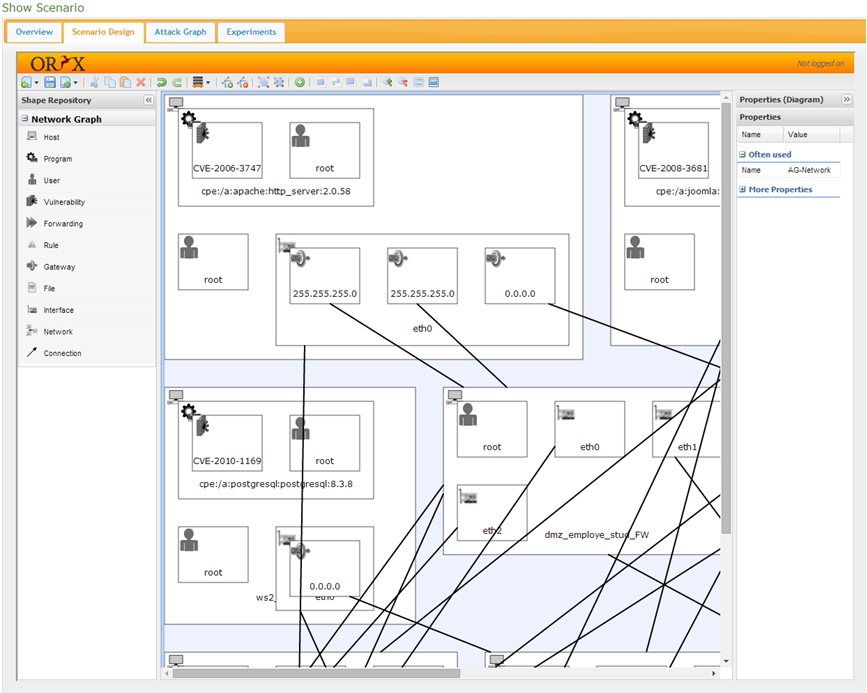
\includegraphics[width=\textwidth]{slg.png}
\caption{SLG}
\label{overflow}
\end{figure}



SLG could be used in several use cases, but the main purpose is providing the platform for teaching and researching of network security. For example, it could be used for Capture The Flag (CTF) seminars. The idea of the seminar is that the tutor deploys potentially vulnerable network with vulnerable applications. Students, in turn, are trying to gain access to the network and to the virtual machines using the found vulnerabilities to find flags. The flag is some label or code. The SLG should provide capability not only to deploy the network environment, but also monitor user activities, find out hacked machines, report on ways of hacking the system, but theses features do not implemented yet. 
  
  
In the this section we just learned Security Lab Generator. On the next section we will introduce OpenStack technologies and the proposal of migrating SLG into the Cloud as a new project CloudSLG in the section "4.4 Security Lab Generator based on OpenStack". 


 

%The current state of the project does not allow to use it for real seminar. SLG requires %implementation of some necessary features. 





%\end{document} 